%%%%%%%%%%%%%%%%%%%%%%%%%%%%%%%%%%%%%%%%%%%%%%%%%%%%%%%%%%%%%%%
%
%     filename  = "main.tex",
%     version   = "1.0.0",
%     authors   = "Ade Irawan",
%     email     = "adeirawan@universitaspertamina.ac.id"
%
%%%%%%%%%%%%%%%%%%%%%%%%%%%%%%%%%%%%%%%%%%%%%%%%%%%%%%%%%%%%%%%
%
% Gunakan skripsistyle.cls dan compile dengan pdflatex.
%
%%%%%%%%%%%%%%%%%%%%%%%%%%%%%%%%%%%%%%%%%%%%%%%%%%%%%%%%%%%%%%%
%
%  2020/01/06   Created  Ade
%  2020/02/05   V1       Ade
%
%%%%%%%%%%%%%%%%%%%%%%%%%%%%%%%%%%%%%%%%%%%%%%%%%%%%%%%%%%%%%%%

\documentclass{skripsistyle}
%\usepackage{showframe} % for showing the frame
\usepackage{lipsum} % for generating dummy text

\usepackage{amsmath}
\usepackage{amssymb}
\usepackage{upgreek}
\usepackage{times}
\usepackage{graphicx}
\usepackage{fancyhdr}
\usepackage{sectsty}
\usepackage{indentfirst}
\usepackage{longtable}
\usepackage{tabularx}
\usepackage{hyperref}
 \usepackage{natbib} % Bibliography with APA Style
\usepackage{geometry}
 \geometry{
 a4paper,
 left=3cm,
 top=2.5cm,
 bottom=2.5cm,
 right=2.5cm,
 }
 
\setlength{\footskip}{1.7cm}
%% Line Spacing
\linespread{1.103} % Jangan dihapus. Ini untuk memastikan line spacing ~15pt. Cara pengecekan: ketik "\the\baselineskip" di dalam dokumen
%% Paragraph spacing
\setlength{\parskip}{9pt}
%% Title
\usepackage{titlesec}
\usepackage{apptools}
\titleformat{\chapter}[display]{\fontsize{14}{14} \center\bfseries}{\IfAppendix{LAMPIRAN}{BAB} \thechapter}{0pt}{}{}
\titleformat{\section}
  {\fontsize{12}{12}\bfseries}{\thesection}{1em}{}
  
\titlespacing*{\chapter}{0pt}{0pt}{1em}
\titlespacing*{\section}{0pt}{0pt}{0pt}

%% Page number
\pagestyle{fancy}
\fancyhf{}
\rfoot{Universitas Pertamina \hspace{1pt}-\hspace{1pt} \thepage}

% Redefine the plain page style
\fancypagestyle{plain}{%
  \fancyhf{}%
\rfoot{Universitas Pertamina \hspace{1pt}-\hspace{1pt} \thepage}%
}

\renewcommand{\headrulewidth}{0pt}
\DeclareMathOperator*{\argmin}{arg\,min}

%------------------------------------------------------------
% Semua informasi penting yang diperlukan
%------------------------------------------------------------
\title{Judul Laporan}{}% {Judul} dan {sub judul jika ada}. Jika tidak ada sub judul biarkan {} kosong
\titleeng{Title}{}% {Judul} dan {sub judul jika ada} dalam bahasa inggris
\author{Penulis}{10521600x} % Nama Penulis dan NIM
\fakultas{Sains dan Ilmu Komputer}
\prodi{Ilmu Komputer}
\tgllulus{15}{Januari 2020} % Tanggal dan bulan+tahun dipisah
\tglpengesahan{29 Januari 2020} % Tanggal, bulan, dan tahun digabung
\tglpernyataan{29 Januari 2020} % Tanggal, bulan, dan tahun digabung
\pembimbingsatu{Ade Irawan, Ph.D.}{116xxx} % Nama dan NIP
\pembimbingdua{Pembimbing Dua}{116xxx} % Nama dan NIP
%\pengujisatu{Randi Farmana Putra, M.Si.}{119030} % Nama dan NIP
%\pengujidua{Herminarto Nugroho, M.Sc.}{116056} % Nama dan NIP
\kaprodi{Nama Kaprodi}{116xxx} % Nama dan NIP
%------------------------------------------------------------

%------------------------------------------------------------
% Uncomment command di bawah ini untuk menambahkan watermark
%------------------------------------------------------------
\usepackage{background} % for adding watermark
\backgroundsetup{anchor = left, hshift = -4.4cm, scale = 1, angle = 0, opacity = 1,
         contents = {
\includegraphics[width = \paperwidth,
         height = 0.9\paperheight, keepaspectratio] {watermark.jpeg}}}

%% Pemecahan suku kata
\hyphenation{me-ning-kat-kan di-tu-lis-kan me-ne-ri-ma me-la-lu-i Na-mun or-ga-ni-sa-i pe-ner-je-mah pe-me-rin-tah me-nge-na-li aug-men-ta-tion meng-gu-na-kan di-gu-na-kan learn-ing trans-fer-ing bi-sin-do}

\begin{document}

\frontmatter
\upcoverpage
\abstrakind{Front/abstrakind}
\abstrakeng{Front/abstrakeng}
\katapengantar{Front/katapengantar}
\daftarisi
\daftartabel
\daftargambar

\mainmatter
%% Chapters
%\renewcommand{\thefootnote}{\arabic{footnote}}
\chapter{PENDAHULUAN}
\label{BAB1:pendahuluan}

\section{Latar Belakang}
\lipsum[1-2]

\section{Rumusan Masalah}
\lipsum[3]

\section{Hipotesis}
\lipsum[4]

\section{Batasan Masalah}
\lipsum[5]

\section{Tujuan Penelitian}
\lipsum[6]


\section{Manfaat Penelitian}
\lipsum[7]

%\section{Waktu Pelaksanaan Penelitian}
%\lipsum[8]


%\renewcommand{\thefootnote}{\arabic{footnote}}
\chapter{TINJAUAN PUSTAKA}
\label{BAB2:tinjauan}

\lipsum[3-4]
\begin{equation}
  L(x,W)= \frac{1}{N}\sum\limits_{i=0}^{N} l(x_i,W)   
  \label{func:loss}
\end{equation}

\lipsum[5-6]
\begin{table}[h]
    \centering
    \caption{Rata-rata loss dan accuracy Model A untuk seluruh round}
\begin{tabularx}{0.95\textwidth} { 
  | >{\centering\arraybackslash}X 
  | >{\centering\arraybackslash}X | }
 \hline
  train\_accuracy &	0.46846 \\
 \hline
  train\_loss &	2.71451 \\
 \hline
  val\_accuracy &	0.47391 \\
  \hline
  val\_loss & 2.69424 \\
  \hline
\end{tabularx}
    \label{tab:my_label}
\end{table}

\lipsum[7]
\begin{center}
\begin{figure}[h]
    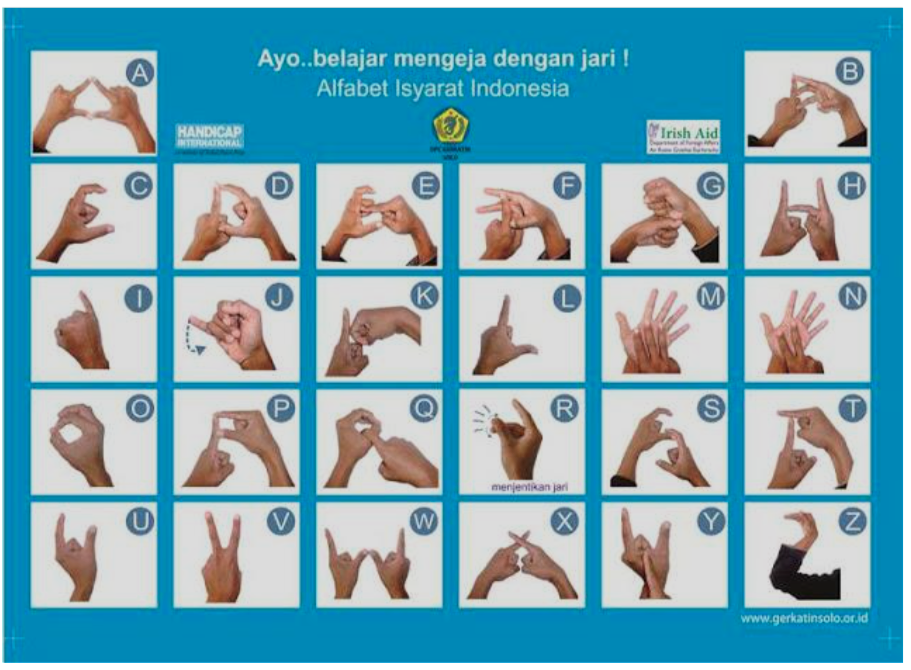
\includegraphics[width=\textwidth]{BAB-2/figures/alfabetbisindo.png}	
	    \caption{Alfabet Bisindo (Almuharram, 2013).}
	    \label{gambar:alfabet bisindo}
\end{figure}
\end{center}
Gambar \ref{gambar:alfabet bisindo} menyunjukkan sudut pandang umum yang digunakan dalam berkomunikasi menggunakan bahasa isyarat, yaitu tampak depan \citep{xiong2004_dscForSensorNetworks}. Sehingga, data gambar yang digunakan di penelitian ini juga memuat gestur Bisindo dari tampak depan, dengan persamaan~(\ref{func:loss}), dengan hasil penelitian di Bab~\ref{BAB4:hasil}.
\chapter{METODE PENELITIAN}
\label{BAB3:Metode}

\lipsum[1-2]
\chapter{HASIL DAN PEMBAHASAN}
\label{BAB4:hasil}

\lipsum[3-4]

\chapter{KESIMPULAN DAN SARAN}

\section{Kesimpulan}
\lipsum[6]

\section{Saran}
\lipsum[9]

%% Appendices
\appendix
\Appendix{Empirical Binary Entropies for Given Bit-Flipping Probabilities}
\label{AppendixA:binaryEntropies}

With simulation setup given in Figure~\ref{fig:p_abc}, the empirical binary entropies for given bit-flipping probabilities are shown in Figure~2 \citep{xiong2004_dscForSensorNetworks}.
\begin{figure}[h]
\centering 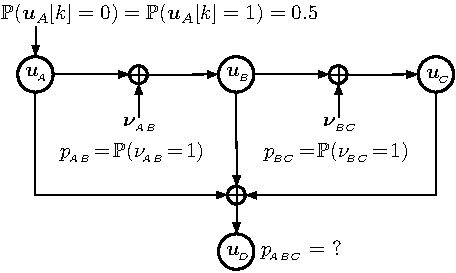
\includegraphics[scale=1]{Lampiran-A/figures/binaryEntropiesSystemSetup-eps-converted-to.pdf}
  \caption{System setup for obtaining $p_{ABC}$.}
  \label{fig:p_abc}	
\end{figure}
% tambahkan sendiri folder-folder (lampiran) yang lain

%------------------------------------------------------------
% BIBLIOGRAPHY %
%------------------------------------------------------------
\begin{singlespace}
  \bibliographystyle{apalike}
  \addcontentsline{toc}{chapter}{DAFTAR PUSTAKA}
  %\addcontentsline{toc}{chapter}{Index}
  \bibliography{Referensi}
\end{singlespace}
\backmatter

\end{document}